\documentclass[11pt]{article}
\usepackage[margin=1in]{geometry}
\usepackage[T1]{fontenc}
\usepackage{newtxtext,newtxmath}
\usepackage{microtype}
\usepackage{graphicx}
\usepackage{booktabs}
\usepackage{tabularx}
\usepackage{enumitem}
\usepackage[font=small,labelfont=bf,skip=4pt]{caption}
\usepackage{titlesec}
\usepackage{xcolor}
\usepackage{tikz}
\usetikzlibrary{positioning,arrows.meta,fit}
\usepackage[hidelinks]{hyperref}

\titleformat{\section}{\normalfont\large\bfseries}{\thesection}{0.6em}{}
\titlespacing*{\section}{0pt}{7pt plus 2pt}{3pt}
\setlist{nosep,leftmargin=1.3em}
\setlength{\parskip}{2pt}
\setlength{\parindent}{0pt}
\setlength{\textfloatsep}{8pt plus 2pt}
\setlength{\floatsep}{6pt plus 2pt}
\setlength{\intextsep}{4pt plus 2pt}
\definecolor{own}{HTML}{0072B2}
\definecolor{other}{HTML}{E69F00}
\definecolor{ink}{HTML}{1F2933}
\definecolor{soft}{HTML}{EEF2F6}

% Team line: edit the roles here.
\newcommand{\teamname}{Team CaptionBench}
\newcommand{\roles}{Jack Hunter (models, scoring code, analysis) \textbullet{}
  Ben Zazycki (role to confirm) \textbullet{} Michael Popov (role to confirm)}

\begin{document}
\pagestyle{plain}

\begin{center}
{\Large\bfseries How Much of a Caption Score Needs the Image?\\[1pt] A Grounding-Gap Study on Flickr8k}\\[4pt]
{\normalsize \teamname{} \textbullet{} CSE 434/534 Midterm Check-In \textbullet{} November 13, 2026}\\[1pt]
{\small \roles}
\end{center}
\vspace{-8pt}

\section{Project Overview}

\textbf{Research question.} A caption metric can reward two different things.
One is wording that fits the dataset in general. The other is content that fits
the one image. We ask two questions. \emph{How much of each automatic caption score can a model
earn without its own image? How does that share change from a model trained
from scratch, to a pretrained model, to a fine-tuned model?}

\textbf{Motivation.} Our proposal planned a comparison of pretrained captioners
on Flickr8k. The first results showed a problem with that plan. BLEU-4 ranked
BLIP base above BLIP large, and three other metrics ranked them the opposite way
(Table~\ref{tab:results}). We therefore changed the object of study from the models to the metrics. We
score every caption twice, once on its own image and once on a different image.
The second score needs no visual grounding, so it measures what the metric pays
for dataset wording alone. Prior work tested metrics with distractor captions
[2] and with object hallucination counts [3].
We found no study that reports this share per metric across training regimes,
but our search was short.

\textbf{Link to course topics.} The study uses convolutional features
(ResNet18) and attention-based Transformer decoders that we train from scratch.
It also uses pretrained vision-language models (BLIP), transfer learning by
fine-tuning, and evaluation design with held-out data.

\section{Dataset}

\textbf{Source and size.} Flickr8k [1] pairs each photo with five
English captions from crowd workers. We use the original split files: 6,000
training, 1,000 validation, and 1,000 test images (40,000 captions).

\textbf{Preprocessing.} The importer rejects an image that appears in two
splits, and it requires five nonempty captions per image. Scoring lowercases
text and uses NLTK WordPunct tokens. Each pretrained model uses its own image
processor. The custom decoders read a cached $7\times7\times512$ ResNet18 grid
per image and a 4,448-word vocabulary (training words seen at least twice).

\textbf{Held-out design.} We divided the validation split once (seed 20261022)
into 800 \emph{search} images and 200 \emph{confirmation} images. Search images
select hyperparameters and epochs. All numbers in this report use the 200
confirmation images. The 1,000 test images stay sealed until the final report.

\textbf{Ethics.} The photos show people who did not consent to model training,
and the captions carry the annotators' guesses about gender and age. The
repository therefore stores aggregate scores only, with no photo and no
reference caption. A high score here is not evidence that captions are
adequate for blind or low-vision readers.

\section{Methods}

\begin{figure}[h]
\centering
\resizebox{\textwidth}{!}{%
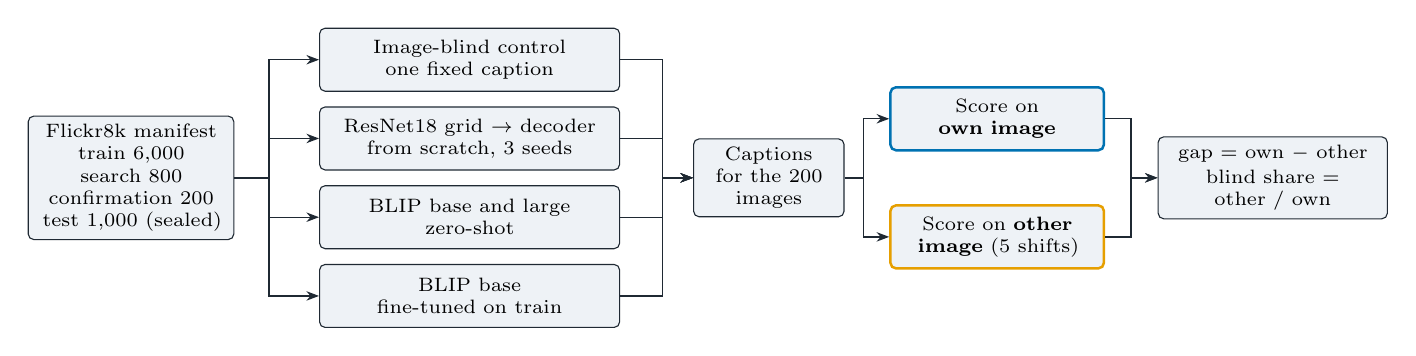
\begin{tikzpicture}[font=\scriptsize, node distance=3mm and 5mm,
  box/.style={draw=ink, rounded corners=2pt, fill=soft, align=center, inner sep=3pt, minimum height=8mm},
  arr/.style={-{Stealth[length=1.6mm]}, draw=ink, line width=0.5pt}]
\node[box, text width=24mm] (data) at (0,0) {Flickr8k manifest\\train 6,000\\search 800\\confirmation 200\\test 1,000 (sealed)};
\node[box, text width=36mm] (blind) at (4.3,1.5) {Image-blind control\\one fixed caption};
\node[box, text width=36mm] (dec) at (4.3,0.5) {ResNet18 grid $\rightarrow$ decoder\\from scratch, 3 seeds};
\node[box, text width=36mm] (blip) at (4.3,-0.5) {BLIP base and large\\zero-shot};
\node[box, text width=36mm] (ft) at (4.3,-1.5) {BLIP base\\fine-tuned on train};
\node[box, text width=17mm] (cap) at (8.1,0) {Captions for the 200 images};
\node[box, text width=25mm, draw=own, line width=0.9pt] (own) at (11.0,0.75) {Score on\\\textbf{own image}};
\node[box, text width=25mm, draw=other, line width=0.9pt] (oth) at (11.0,-0.75) {Score on \textbf{other}\\\textbf{image} (5 shifts)};
\node[box, text width=27mm] (gap) at (14.5,0) {gap $=$ own $-$ other\\[1pt]blind share $=$\\other / own};
\foreach \m in {blind,dec,blip,ft} {\draw[arr] (data.east) -- (1.75,0) |- (\m.west); \draw[arr] (\m.east) -- (6.75,0 |- \m.east) |- (cap.west);}
\draw[arr] (cap.east) -- (9.3,0) |- (own.west);
\draw[arr] (cap.east) -- (9.3,0) |- (oth.west);
\draw[arr] (own.east) -- (12.7,0.75) |- (gap.west);
\draw[arr] (oth.east) -- (12.7,-0.75) |- (gap.west);
\end{tikzpicture}}
\caption{System design. One scorer rates each caption on its own image and on other images.}
\label{fig:system}
\end{figure}

The unit of analysis is one caption for one confirmation image ($n=200$ per
model). Figure~\ref{fig:system} shows the design. The protocol has four steps.

\begin{enumerate}[leftmargin=1.5em,itemsep=2pt]
\item \textbf{Generate captions under four conditions.}
(a) \emph{Image-blind control}: the fixed caption ``a photo of a person in a scene''.
(b) \emph{Decoders from scratch}: a two-layer Transformer decoder (width 128,
four heads, 1.6M parameters) attends over the 49 cells of a frozen ResNet18
grid. The \emph{relation} variant adds self-attention among the cells. Training used AdamW (learning rate $9\times10^{-4}$ plain, $1.2\times10^{-3}$ relation;
batch 128, 12 epochs), the best epoch by search-set loss, greedy decoding, and
seeds 17, 29, and 43.
(c) \emph{Zero-shot BLIP} [4]: the released base and large captioning
checkpoints, with three beams and at most 32 new tokens.
(d) \emph{Fine-tuned BLIP base}: all weights, AdamW (learning rate $10^{-5}$,
weight decay 0.05, batch 8), a one-cycle cosine schedule, and two epochs
over the 30,000 training pairs. Decoding is the same as in (c).
\item \textbf{Score on the own image.} One scorer computes corpus BLEU-4
[5], METEOR [6], CIDEr-D [7],
and reference-free CLIPScore [8] (CLIP ViT-B/32). We wrote
CIDEr-D ourselves. It agrees with the \texttt{pycocoevalcap} reference to
$10^{-15}$ per image on 12 prediction files.
\item \textbf{Score on other images.} We sort the 200 image IDs. For each shift
$s \in \{1, 37, 73, 109, 151\}$, caption $i$ is scored against the references
and pixels of image $(i+s) \bmod 200$. The \emph{other-image} score is the mean
over the five shifts. CIDEr-D document frequencies do not change, because the
reference set is the same.
\item \textbf{Derive two quantities.} The \emph{grounding gap} is the own-image
score minus the other-image score. The \emph{blind share} is the other-image
score divided by the own-image score. A blind share of 100\% means that the
metric cannot tell whether the model saw the image.
\end{enumerate}

\textbf{Uncertainty.} Intervals are 95\% percentile bootstraps over images
(2,000 resamples).
\textbf{What we fixed in advance.} We froze the validation partition and the
decoder configurations on October 22, before any confirmation score. We
designed the other-image analysis on November 11, after we saw the BLIP rank
reversal. That analysis is therefore exploratory.

\section{Preliminary Results}

\begin{table}[h]
\centering\small
\setlength{\tabcolsep}{4.2pt}
\begin{tabular}{@{}l rr rr rr rr r@{}}
\toprule
 & \multicolumn{2}{c}{BLEU-4} & \multicolumn{2}{c}{METEOR} & \multicolumn{2}{c}{CIDEr-D} & \multicolumn{2}{c}{CLIPScore} & \\
\cmidrule(lr){2-3}\cmidrule(lr){4-5}\cmidrule(lr){6-7}\cmidrule(lr){8-9}
Condition & own & blind\,\% & own & blind\,\% & own & blind\,\% & own & blind\,\% & tokens \\
\midrule
\csname @@input\endcsname results-table.tex
\bottomrule
\end{tabular}
\caption{The 200 confirmation images. \emph{own}: score on the caption's own
image (BLEU-4, METEOR $\times100$; CIDEr-D 0--10; CLIPScore 0--2.5).
\emph{blind\,\%}: share of that score kept on other images. \emph{tokens}: mean caption length.}
\label{tab:results}
\end{table}

\begin{figure}[h]
\centering
\includegraphics[width=0.93\textwidth]{figures/blind-share.pdf}
\caption{Own-image and other-image scores. The label above each pair is the blind share.}
\label{fig:blind}
\end{figure}

\textbf{1. The metrics disagree about the two released models.} BLEU-4 puts
BLIP base first (22.9 against 20.5). METEOR, CIDEr-D, and CLIPScore put BLIP
large first. The outputs show one cause. BLIP large starts 182 of its 200
captions with ``there is'' or ``there are''. Only 203 of the 30,000 training
references start that way. Its captions are also twice as long.

\textbf{2. The metrics differ in how much they pay without the image.} For
zero-shot BLIP base, a caption keeps 8\% of its CIDEr-D on another image, 14\%
of its BLEU-4, 41\% of its METEOR, and 65\% of its CLIPScore. The fixed control
caption gets a CLIPScore of 0.54 and the best model 0.81, a narrow usable range.

\textbf{3. The blind share falls along the training ladder.} The decoders that
we trained from scratch keep 27\% of their BLEU-4 on other images. Zero-shot
BLIP keeps 10--14\%, and fine-tuned BLIP keeps 10\%. The same order holds for
CIDEr-D (15\%, 7--8\%, 5\%) and CLIPScore (67\%, 60--65\%, 53\%). A small model
trained only on Flickr8k learns the dataset's wording before it learns to
ground it. The order survives a harder test: each photo paired with its most
similar photo (optimal matching on CLIP image similarity). The decoders then
keep 62--65\% of their CIDEr-D, zero-shot BLIP 30--34\%, and fine-tuned BLIP 24\%.

\textbf{4. Fine-tuning gains are mostly grounded. Our hypothesis was wrong.}
We expected fine-tuning to raise scores mainly through Flickr8k wording.
Fine-tuning raised BLEU-4 from 22.9 to 35.5 and CIDEr-D from 0.55 to 1.10
(95\% interval 1.00--1.20). The other-image score supplied only 2 of the 55
percentage points of relative BLEU-4 gain, and 2 of 99 for CIDEr-D. CLIPScore
rose from 0.72 to 0.81 while its other-image score fell from 0.47 to 0.43.
METEOR is the exception: 21 of its 66 points of relative gain appear on other
images too. One fine-tuning seed supports these numbers.

\textbf{5. The relation layer did not help (negative result).} It reached
17.5 BLEU-4 against 18.1 for the plain decoder (three seeds each). The paired
bootstrap interval, $[-2.08, 0.60]$ points, includes zero. We stop that work.

\begin{table}[h]
\centering\footnotesize
\begin{tabular}{@{}ll@{}}
\toprule
Decoder, plain & a woman in a black shirt is sitting on a cellphone with a \textless unk\textgreater{} in a crowd \\
BLIP base & a woman holding a sign \\
BLIP large & there are two women holding a sign that says free hugs \\
BLIP base, fine-tuned & two girls hold up a yellow sign that says, i love you, happy, free hugs \\
\bottomrule
\end{tabular}
\caption{Outputs for one confirmation photo: two women hold signs that offer
free hugs (our description). The fine-tuned model adds detail and invents sign text.}
\label{tab:examples}
\end{table}

\textbf{Limits.} The set has 200 photos, and fine-tuning has one seed. The
shares depend on how similar Flickr8k photos are, so they do not transfer to
another dataset. No human rating supports any metric yet.

\section{Next Steps}

\textbf{Planned improvements.}
(1) Repeat fine-tuning with three seeds, and record the blind share after every
500 steps.
(2) Move training to Colab. One notebook runs every stage, and adds a decoder on ConvNeXt features and a fine-tuned BLIP large.
(3) Add BERTScore and BLIP-2.

\textbf{Evaluation strategy.}
(1) We freeze this protocol and run it once on the 1,000 sealed test images.
(2) Flickr8k includes 5,822 expert judgments of caption-image pairs. We will
test whether a metric with a low blind share agrees better with them.
(3) Three team raters will score 100 photos on our tested, blinded rating forms.

\textbf{Open questions.}
Does a low blind share predict agreement with human ratings, or only
sensitivity to n-grams? Does the fine-tuned model
hallucinate more detail (Table~\ref{tab:examples}), and does any of the four metrics penalize it?

\vspace{3pt}\hrule\vspace{3pt}
{\footnotesize\textbf{References.}
[1]~Hodosh et al. Framing image description as a ranking task. \emph{JAIR}, 2013.
[2]~Kilickaya et al. Re-evaluating automatic metrics for image captioning. \emph{EACL}, 2017.
[3]~Rohrbach et al. Object hallucination in image captioning. \emph{EMNLP}, 2018.
[4]~Li et al. BLIP: bootstrapping language-image pre-training. \emph{ICML}, 2022.
[5]~Papineni et al. BLEU: a method for automatic evaluation of machine translation. \emph{ACL}, 2002.
[6]~Banerjee, Lavie. METEOR: an automatic metric for MT evaluation. \emph{ACL Workshop}, 2005.
[7]~Vedantam et al. CIDEr: consensus-based image description evaluation. \emph{CVPR}, 2015.
[8]~Hessel et al. CLIPScore: a reference-free evaluation metric for image captioning. \emph{EMNLP}, 2021.
\par}

\clearpage
\thispagestyle{empty}
\newgeometry{margin=0.4in}
\thispagestyle{empty}
\noindent\makebox[\textwidth][c]{\includegraphics[height=10.1in]{figures/gallery.pdf}}

\end{document}
